The application architecture has three logic layer that describes below:
\begin{itemize}
    \item \textbf{Presentation layer (P)} The presentation tier is the front end layer in the 3-tier system and consists of the user interface. This user interface is often a graphical one accessible through a web browser or web-based application and which displays content and information useful to an end user.\\
    
    \item \textbf{Application layer (A)}  is the heart of the application. This layer contains the functional business logic which drives an application’s core capabilities. the layer where all your business logic resides is the application layer.\\
    
    \item \textbf{Data access layer (D)} comprises of the database/data storage system and data access layer. It picks up useful information for the users in the database and passes them along the other layers.\\
\end{itemize}

There are many benefits to using a 3-layer architecture including speed of development, scalability, performance, and availability.  As mentioned, modularizing different tiers of an application gives development teams the ability to develop and enhance a product with greater speed than developing a singular code base because a specific layer can be upgraded with minimal impact on the other layers.  It can also help improve development efficiency by allowing teams to focus on their core competencies. Many development teams have separate developers who specialize in front- end, server back-end, and data back-end development, by modularizing these parts of an application you no longer have to rely on full stack developers and can better utilize the specialties of each team.\\

\begin{figure}[H]
  \centering
  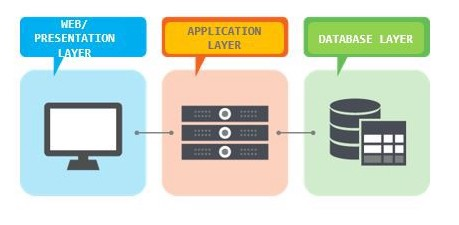
\includegraphics[width=0.6\textwidth,keepaspectratio]{images/all/3tier.jpg}
  \caption{Three-tier architecture}
\end{figure}

the chief benefit of three-tier architecture its logical and physical separation of functionality. Each tier can run on a separate operating system and server platform - e.g., web server, application server, database server - that best fits its functional requirements. And each tier runs on at least one dedicated server hardware or virtual server, so the services of each tier can be customized and optimized without impact the other tiers.
some benefits of three tier development are: 
\begin{itemize}
    \item Faster development
    \item Improved scalability
    \item Improved reliability
    \item Improved security
\end{itemize}